\documentclass[a4paper,12pt]{ctexrep}
\usepackage{float}
\usepackage{subcaption}
\usepackage{amsmath}
\usepackage{color}

\begin{document}
	% top matter
	\title{\textbf{MWDC宇宙线标定测试平台用户指南}}
	\author{周勇,唐述文\\
	次级束物理研究组\\
	中国科学院近代物理研究所\\
	\texttt{yong@impcas.ac.cn, zyong06@gmail.com}}

	\maketitle

	% article and report can have an abstract
	\begin{abstract}
	MWDC宇宙线标定测试平台是一套完整的宇宙线刻度系统,它由以下几个部分组成:大真空靶室及其辅助真空设备,径迹探测器分系统,触发探测器分系统,数据获取分系统(DAQ)以及离线分析软件。

	该测试平台最初是基于暗物质粒子探测卫星(DAMPE)塑闪阵列探测器的地面宇宙线刻度而设计和搭建的,因此其主体框架是一套大真空靶室以及相应的辅助真空设备。测试时,被测探测器放置在真空靶室内部。

	径迹探测器分系统由两个多丝漂移室(MWDC)构成,分别放置在靶室上部和下部,用于确定入射宇宙线的径迹。根据测得的径迹,可以反推出其在被测探测器上的击中位置,从而准确得到探测器的位置响应。

	触发探测器分系统由两个大面积的塑闪板探测器构成,分别放置在上MWDC的上部和下MWDC的下部。它用于标记入射宇宙线事例,为整个平台提供快触发信号和起始时间信号。

	离线分析软件基于ROOT和C++,用于原始数据的解码,数据质量的校验以及数据分析。
	\end{abstract}

	\tableofcontents
	\listoffigures
	\listoftables

	\chapter{探测器部分}

\section{整体布局与坐标系统}


\section{探测器结构}
\subsection{多丝漂移室}

\subsection{大面积塑闪板}

\subsection{探测器编号}

\section{真空靶室与相关设备}



	\chapter{电子学部分}
\section{PXI获取系统与HPTDC简介}

\subsection{HPTDC基本参数}
HPTDC基本参数如表\ref{tbl:hptdc_parameters}所示:
\begin{table}
	\centering
		\begin{tabular}{|l|l|l|p{6cm}|}
			\hline
			参数 & 意义 & 数值 & 备注 \\ 
			\hline
			Bunch ID & 触发信号的时间戳 & 用12 bits存储,单位25ns,范围102.4us &  \\ 
			\hline
			高精度测量的精度 & High Precision Mode & 19 bits, 单位$25/256 ns\simeq 100 ps$,范围51.2us &  \\ 
			\hline
			超高精度测量的精度 & Very High Precision Mode & 21 bits, 单位$25/256/4 ns \simeq 25 ps$ ,范围51.2us & \\
			\hline
			Coarse Time Counter & 用于拓展时间测量量程 & 时钟源来自PLL(40,160,320Hz),共15 bits & 40Hz是使用低12位,160Hz使用低14位,320Hz使用全部15位 \\
			\hline
			DLL & 用于精细时间测量 & 时钟源来自PLL(40,160,320Hz),将一个周期时钟分为32份,等效于5 bits & \\
			\hline
		\end{tabular}
		\caption{HPTDC基本性能参数}
		\label{tbl:hptdc_parameters}
\end{table}

\subsection{HPTDC使用要点}

\section{MWDC读出电子学}

\subsection{通道对应关系}

\section{塑闪板读出电子学}

\subsection{通道对应关系}

\section{触发板与时钟板}

\section{数据格式}

\subsection{Ungrouped格式}
在2015年2、3月份间的测试过程中,原先设计的事件打包逻辑有bug存在,因此正式的宇宙线测试中使用了Ungrouped格式,即使用HPTDC原始的打包格式。具体如下:
\begin{itemize}
	\item 每块获取卡对应一个独立的原始数据文件,文件具有相同的前缀,和后缀“atl”,并使用获取卡所在的槽位编号。
	\item 数据逐事件存储。每个Event的数据由一个Group Header和一个Group Trailer组成的数据段组成;Header和Trailer中间是各块HPTDC的测量数据,且只是各通道的测量数据,而不包含HPTDC的Header和Trailer。每个word的具体格式参考HPTDC说明书。
	\item 对于MWDC来说,获取板上四片HPTDC从0-3编号,读取顺序为3-2-1-0;\textbf{出于未知的原因,MWDC的信号前沿是原始数据中的Trailing Time,而信号后沿是原始数据中的Leading Time。}。
	\item 对于TOF获取板来说,其信号前后沿与原始数据中的Leading/Trailing Time是一致的。
	\item Bunch ID的决定值是与trigger latency相关的,当所有获取卡的trigger latency一致时,同一事件的Bunch ID也应该是一致的;若trigger latency不一致,则Bunch ID的差值就是Trigger Latency的大小。这是因为trigger time tag是要减去trigger latency后才存入Trigger FIFO中的。
\end{itemize}

已知问题:
\begin{enumerate}
	\item 对于单个事例来讲,MWDC获取板上的最大读出数据长度为$256\times4=1024$个word(根据HPTDC的Readout FIFO存储深度计算)。实际测试中发现,偶尔会出现大事例,此时数据长度超过1024个word,但不影响数据格式。
	\item 在正确使用触发板的条件下,不同获取卡间的bunch id基本能够对齐,偶尔会出现$\pm 1$的浮动,但会恢复。
	\item 在正确使用触发板的条件下,每块获取卡内的event id是连续的;基本都能从0开始计数,偶尔会有若干获取卡可能不从0开始。
	\item Group Trailer中的word count是不准确的
	\item Group Header和Group Trailer中的event id是一致的。
\end{enumerate}





	\chapter{分析软件介绍}

\section{配置文件-crate.json}

\section{ROOT输出文件格式}

\begin{table}
	\centering
		\begin{tabular}{|l|p{2cm}|l|p{6cm}|}
			\hline
			Branch Name &  Type & Value & Meaning \\ 
			\hline
			\texttt{event\_flag} &  \texttt{Char\_t}(B) & 1,2,3 & 代表该Event格式是否正确,1是正常情况,2是有Header无Trailer(一般是文件最后一个不完整的事件),3是Header中的EventID不等于Trailer中的EventID \\ 
			\hline
			\texttt{event\_id} & \texttt{Int\_t}(B) & 12 bits & 代表该Event的事件号(来自Master TDC),是直接从数据中解码出来的。由于Group Header和Trailer中都包含EventID,若\texttt{event\_flag=3},则该字段是来自Header\\ 
			\hline
			\texttt{bunch\_id} & \texttt{Int\_t} & 12 bits & 直接从Group Header中解码得到(来自Master TDC)。\\
			\hline
			\texttt{leading\_raw} & \texttt{std::map<Uint\_t,std::vector<int>} & 19 bits & MWDC板的高精度TOT后沿时间测量值,key是面板上的通道编号\\
			\hline
			\texttt{trailing\_raw} & \texttt{std::map<Uint\_t,std::vector<int>} & 19 bits & MWDC板的高精度TOT前沿时间测量值,key是面板上的通道编号 \\
			\hline
			\texttt{time\_leading\_raw} & \texttt{std::map<Uint\_t,std::vector<int>} & 21 bits & TOF板甚高精度TOT前沿时间测量值,key是面板上的通道编号 \\
			\hline
			\texttt{time\_trailing\_raw} & \texttt{std::map<Uint\_t,std::vector<int>} & 21 bits & TOF板的甚高精度TOT后沿时间测量值,key是面板上的通道编号 \\
			\hline
			\texttt{tot\_leading\_raw} & \texttt{std::map<Uint\_t,std::vector<int>} & 19 bits & TOF板的高精度TOT前沿时间测量值,key是面板上的通道编号 \\
			\hline
			\texttt{tot\_trailing\_raw} & \texttt{std::map<Uint\_t,std::vector<int>} & 19 bits & TOF板的高精度TOT后沿时间测量值,key是面板上的通道编号 \\
			\hline
		\end{tabular}
		\caption{每块MWDC卡/TOF卡解码后得到的TTree格式}
		\label{tbl:raw_format}
\end{table}

	\chapter{MWDC的自身刻度}


	\appendix
	\chapter{2015年2、3月份间的宇宙线测试数据分析}

\section{触发时间间隔分布}
\subsection{问题描述}
一般认为宇宙线事例的时间间隔分布满足指数衰减规律,即
\begin{equation}
	P(t) = \frac{1}{T_{interval}}e^{-t/T_{interval}}
\end{equation}
其中,$T_{interval}$是宇宙线事例的平均时间间隔。

\subsection{结果}
对test21文件进行分析得到如下典型结果。这些结果无论是对MWDC板的Bunch ID,还是对TOF板的Bunch ID或Leading Time都是一致的。

\subsubsection*{事件发生的时间戳在测量时间范围内呈均匀分布}
MWDC板和TOF板的Bunch ID在$[0,4095]$呈均匀分布,TOF板的Leading Time在$[0,2097151]$呈均匀分布,典型示例如图\ref{fig:tof_leadingtime_distribution}所示。
\begin{figure}[htbp]
	\centering
	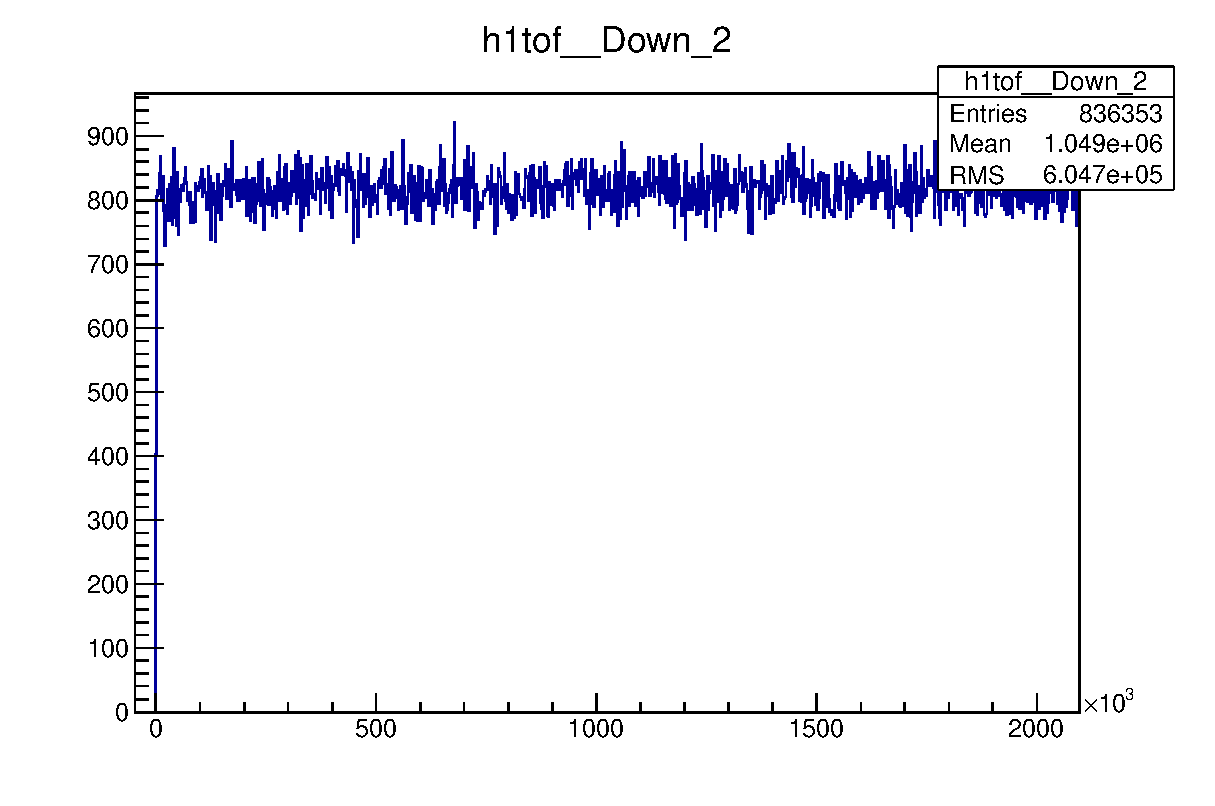
\includegraphics[width=0.95\textwidth]{fig/tof_leadingtime_distribution.eps}
	\caption{TOF板测得的Leading Time原始分布}
	\label{fig:tof_leadingtime_distribution}
\end{figure}

\subsubsection*{前后两个事件的时间戳关联呈统计无关}
MWDC板和TOF板的前后事件间的Bunch ID关联,以及TOF板的Leading Time关联呈统计无关,典型示例如图\ref{fig:tof_leadingtime_current_vs_previous}所示。
\begin{figure}[H]
	\centering
	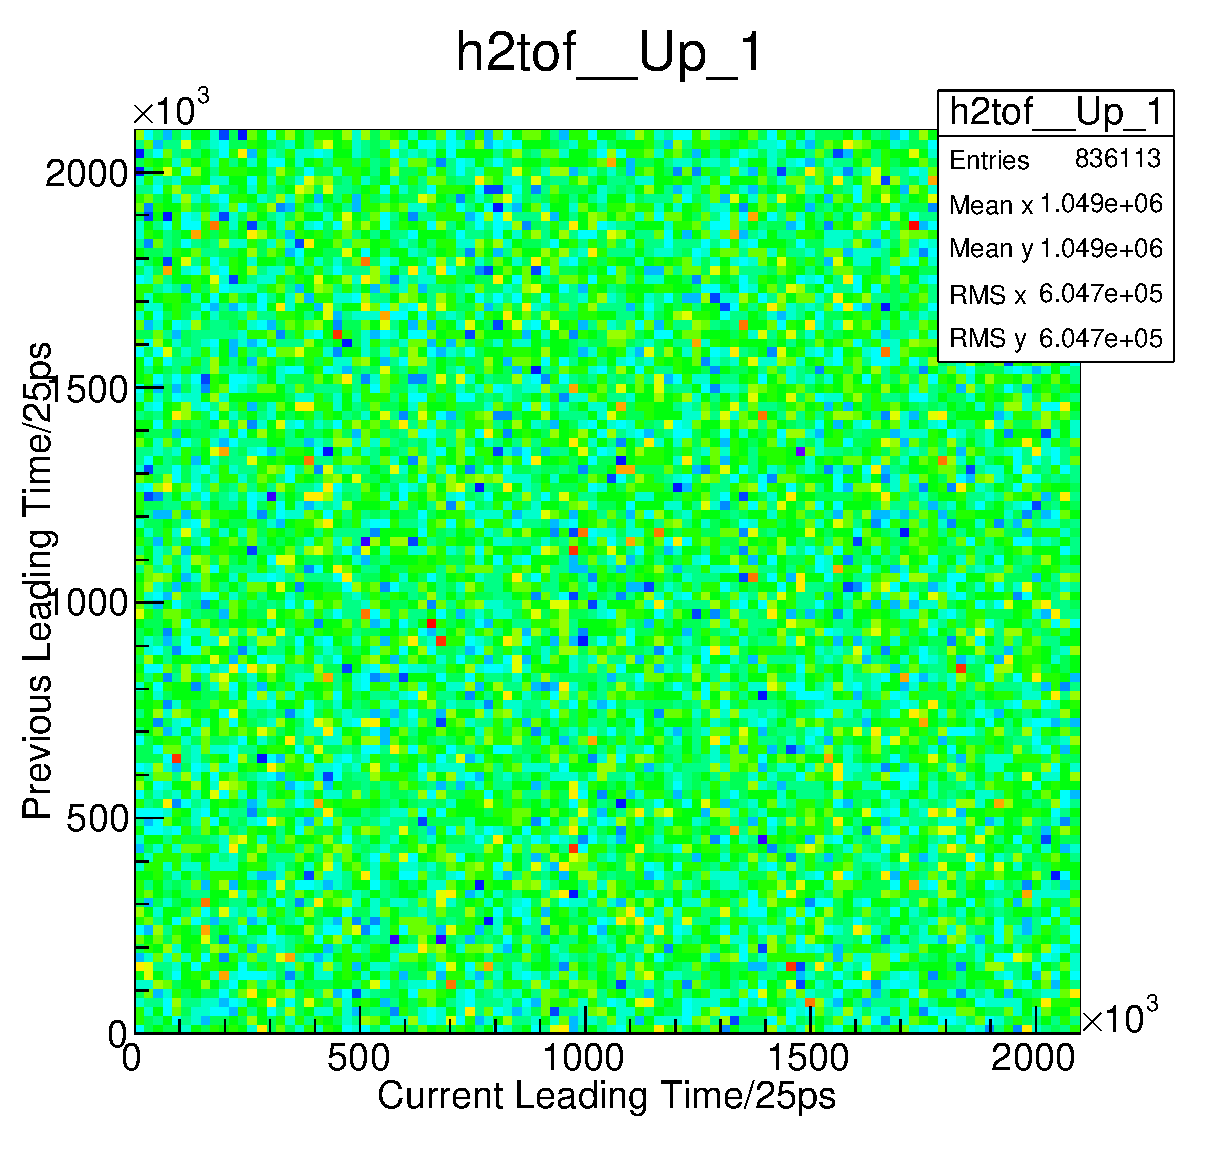
\includegraphics[width=0.8\textwidth]{fig/tof_leadingtime_current_vs_previous.eps}
	\caption{TOF板测得的相邻事件Leading Time的关联性}
	\label{fig:tof_leadingtime_current_vs_previous}
\end{figure}
此结果需要思考,因为实际中,宇宙线事例的时间间隔分布是有一定概率分布的,满足指数衰减规律。而测量结果确模糊了这种关联性。

\subsubsection*{触发时间间隔呈等腰三角形分布}
将前后事件的时间戳(Bunch ID或Leading Time)直接相减得到的触发时间分布呈等腰三角形.
图\ref{fig:bunchid_interval}给出了MWDC和TOF板得到的Bunch ID时间间隔分布。
\begin{figure}[htbp]
	\centering
	\begin{subfigure}[b]{0.48\textwidth}
        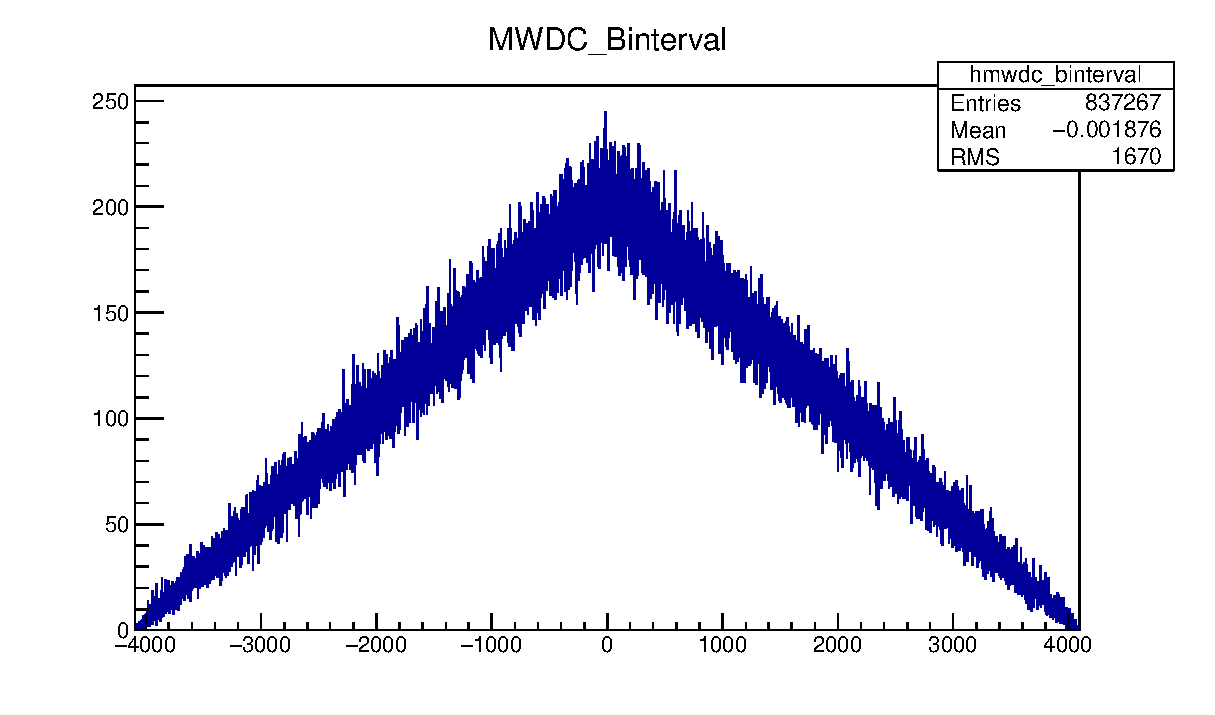
\includegraphics[width=\textwidth]{fig/mwdc_bunchid_interval.eps}
        \caption{MWDC}
        \label{fig:mwdc_bunchid_interval}
    \end{subfigure}
    ~
    \begin{subfigure}[b]{0.48\textwidth}
        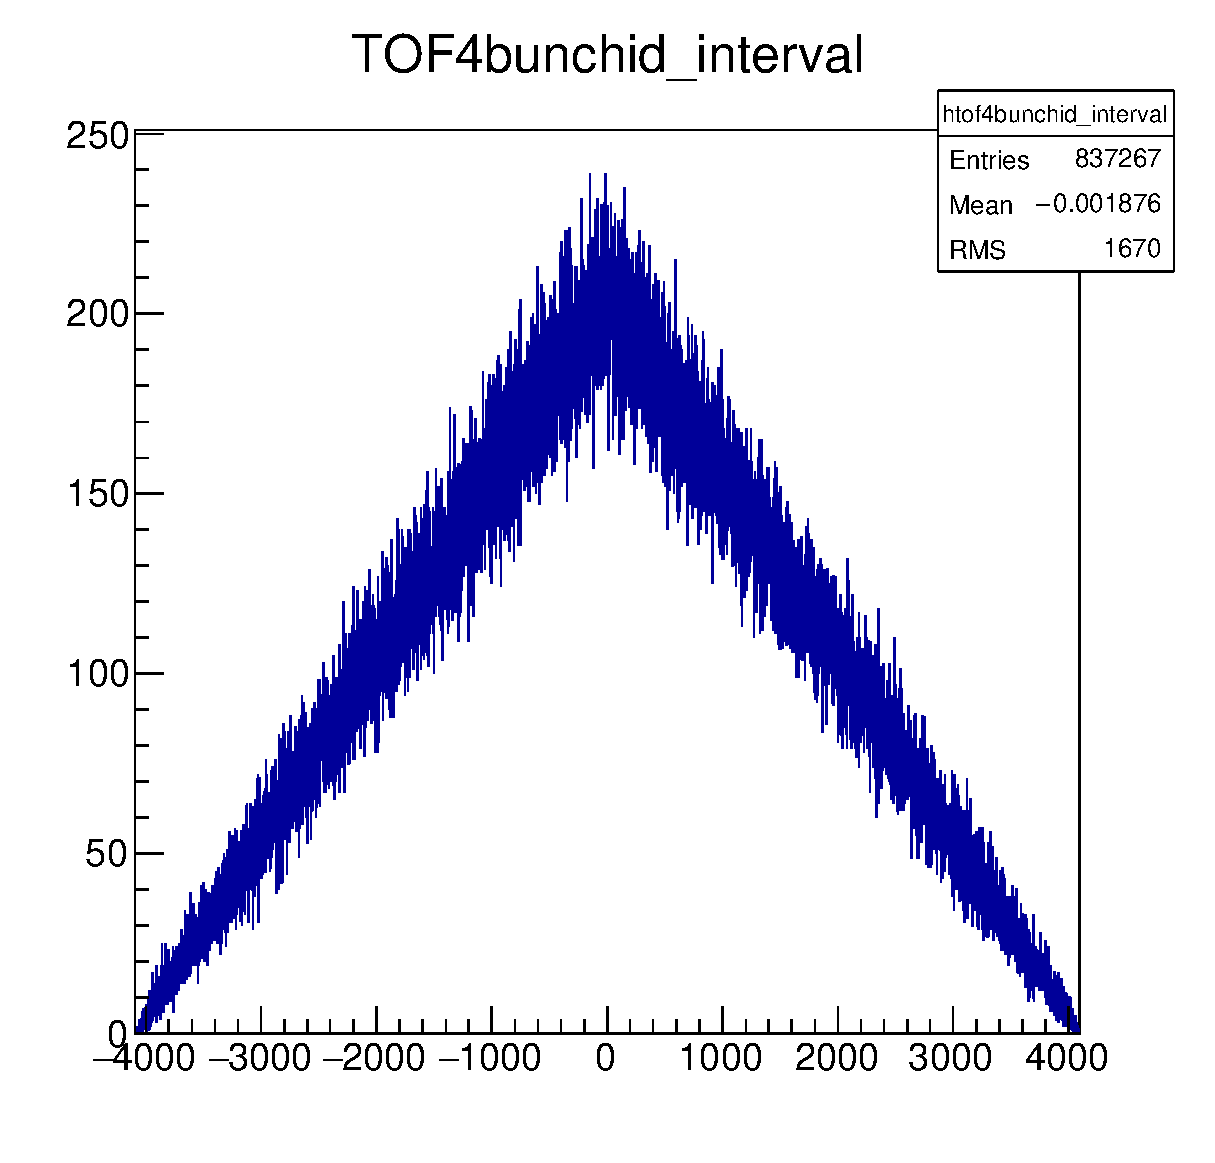
\includegraphics[width=\textwidth]{fig/tof_bunchid_interval.eps}
        \caption{TOF}
        \label{fig:tof_bunchid_interval}
    \end{subfigure}
	\caption{Bunch ID的时间间隔分布}
	\label{fig:bunchid_interval}
\end{figure}

若对时间测量的roll over进行修正,则得到的时间间隔分布在测量范围内是均匀的,如图\ref{fig:tof_interval_rollover}所示。
roll over修正是指:由于时间测量范围有限,时间戳在一定周期后会自动翻转再从0开始,此时后一事件的时间戳可能小于前一事件的时间戳,此时将后一事件的时间戳测量值加上时间测量量程后再进行相减。
\begin{figure}[htbp]
	\centering
	\begin{subfigure}[b]{0.48\textwidth}
        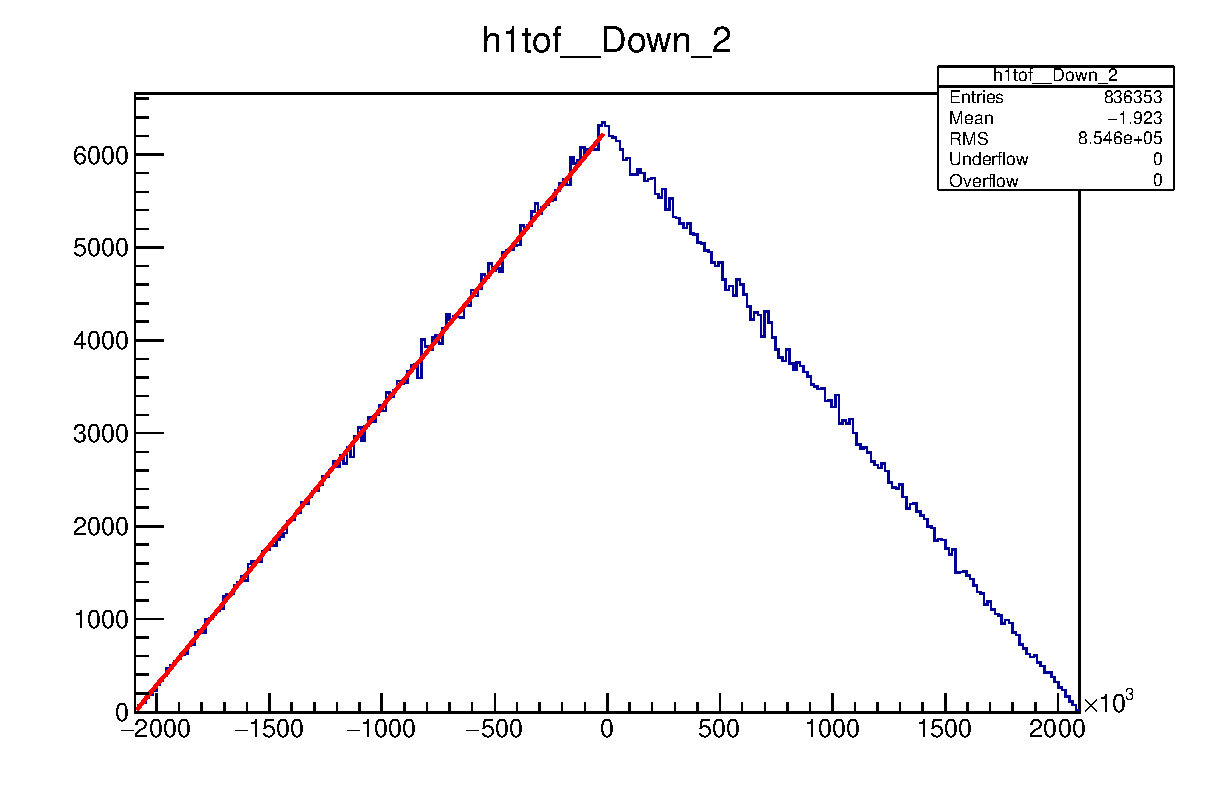
\includegraphics[width=\textwidth]{fig/tof_interval.eps}
        \caption{roll over修正前}
        \label{fig:tof_interval}
    \end{subfigure}
~
    \begin{subfigure}[b]{0.48\textwidth}
        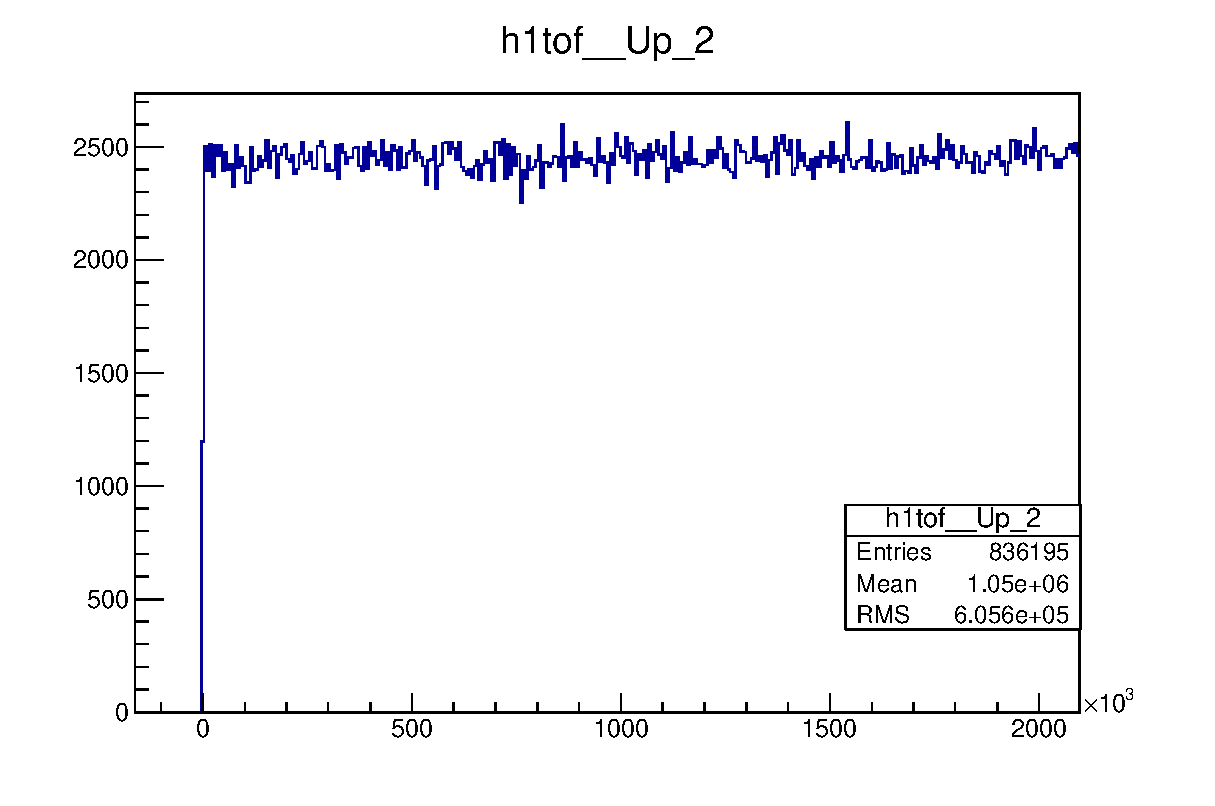
\includegraphics[width=\textwidth]{fig/tof_interval_correct_rollover.eps}
        \caption{roll over修正后}
        \label{fig:tof_interval_correct_rollover}
    \end{subfigure}
	\caption{TOF板得到的Leading Time时间间隔分布在roll over进行修正前后}
	\label{fig:tof_interval_rollover}
\end{figure}

\subsection{讨论}
等腰三角形分布可以用两种方法进行解释:
\subsubsection*{从指数衰减分布出发}
条件:时间间隔$T_{interval}$满足指数衰减分布,时间常数为$\lambda$,且时间测量量程$R\ll\lambda$。在测量量程内的时间戳为$T_{measusred}=T_{real}\mod R$,其中$T_{real}$是实际的时间间隔大小。

根据上述条件可以得到:
\begin{align}
&\begin{cases}
dT_{measured} =dT_{real}\\
\frac{P}{P+dP} = \frac{\sum\limits_{n=0}^{\infty}e^{-(T_{measured}+nR)/\lambda}}{\sum\limits_{n=0}^{\infty}e^{-(T_{measured}+dT_{measured}+nR)/\lambda}}
\end{cases}\\
\Rightarrow &\frac{dP}{P}=-\frac{dT_{measured}}{\lambda}\\
\Rightarrow &P(T_{measured})\propto e^{-\frac{T_{measured}}{\lambda}}, T_{measured}\in[0,R]
\end{align}

进一步考虑roll over对概率分布的影响。
由于时间戳在量程范围内是均匀分布的,因此对于某一确定的$T_{measured}$,其时间间隔为正值所占的比例应该是$\frac{R-T_{measured}}{R}$,为负值的比例应该是$\frac{T_{measured}}{R}$。
由此可以得到,不考虑roll over修正的概率分布为
\begin{equation}
	\begin{cases}
	P(T_{measured})=\frac{R-T_{measured}}{R}e^{-\frac{T_{measured}}{\lambda}} & ,T_{measured}\in[0,R]\\
	P(T_{measured})=\frac{R+T_{measured}}{R}e^{-\frac{T_{measured}+R}{\lambda}} &,T_{measured}\in[-R,0]\\
	\end{cases}
\end{equation}

上式在$R\ll\lambda$时,就是等腰三角形分布,如图\ref{fig:interval_pdf}所示
\begin{figure}[htbp]
	\centering
	\begin{subfigure}[b]{0.48\textwidth}
        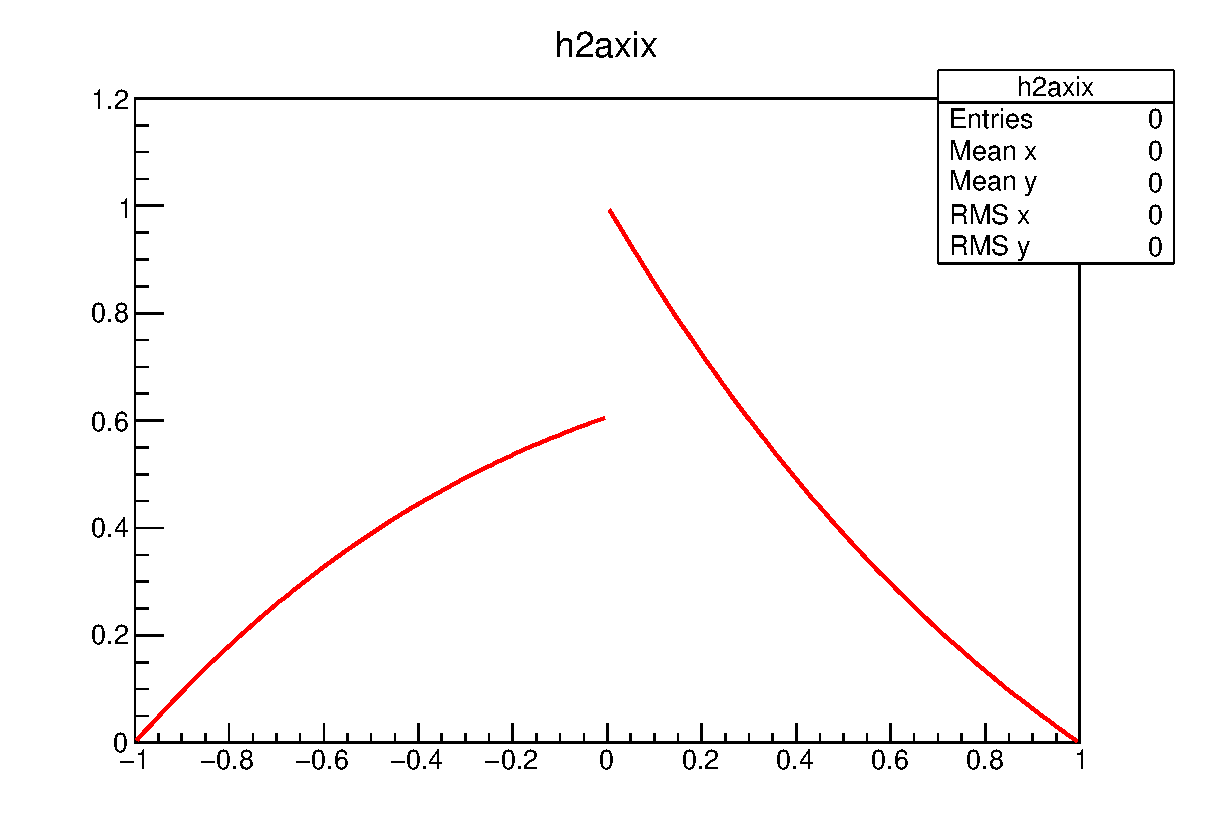
\includegraphics[width=\textwidth]{fig/interval_pdf_largerange.eps}
        \caption{$R\simeq\lambda$}
    \end{subfigure}
    \begin{subfigure}[b]{0.48\textwidth}
        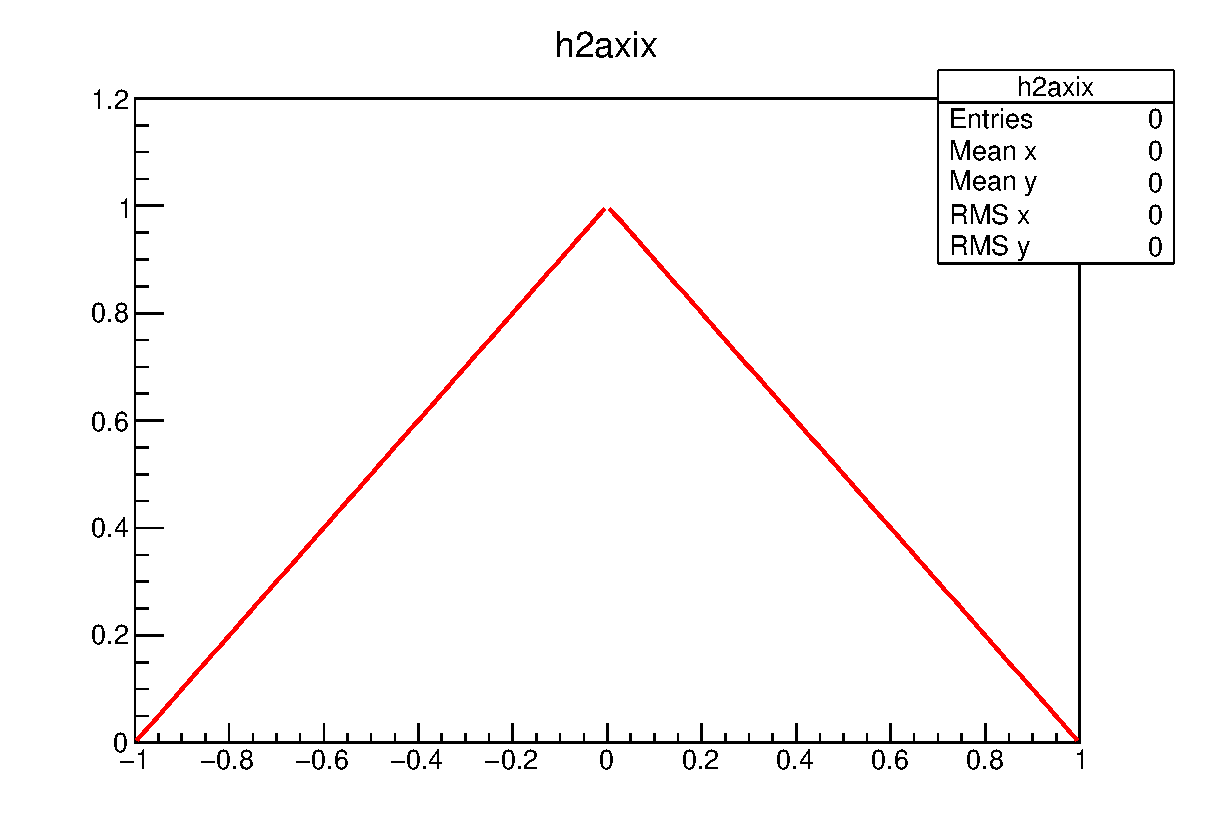
\includegraphics[width=\textwidth]{fig/interval_pdf_smallrange.eps}
        \caption{$R\ll\lambda$}
    \end{subfigure}
	\caption{测量范围从大到小的演化}
	\label{fig:interval_pdf}
\end{figure}


\subsubsection*{从均匀随机分布出发}
由上述结果中得到前后事件的时间戳分别呈均匀分布,且相互独立(无统计关联)。
假设$T_{current}$和$T_{previous}$分布是前后事件的时间戳,它们的取值范围为$[0,R]$,其中R是时间测量量程,而${T_interval=T_{current}+(-T_{previous})}$。令$Z=T_{interval}$,$Y=T_{current}$,$X=-T_{previous}$,则$Z=Y+X$,即随机变量$Z$是两个相互独立的随机变量$X、Y$之和,其中
\begin{align}
P(Y)&=1, Y\in [0,R]\\
P(X)&=1, X\in [-R,0]
\end{align}
两个独立随机变量之和的概率分布是这两个分布的卷积。且对于均匀分布的随机变量来说,其和的概率分布,通过卷积公式计算得到的就是等腰三角形分布,即
\begin{equation}
	\begin{cases}
	P(Z)=Z+R,&(-R\leq Z \leq 0)\\
	P(Z)=R-Z,&(0\leq Z \leq R)
	\end{cases}
\end{equation}

\subsection{遗留问题}
\underline{上述两种解释是否可以统一?}

\section{TOF获取卡Bunch ID与Leading Time之差}
四块TOF获取卡的Bunch ID与Leading Time之间的差值基本都稳定在$10*25=250ns$左右。

\begin{figure}[htbp]
	\centering
	\begin{subfigure}[b]{0.48\textwidth}
        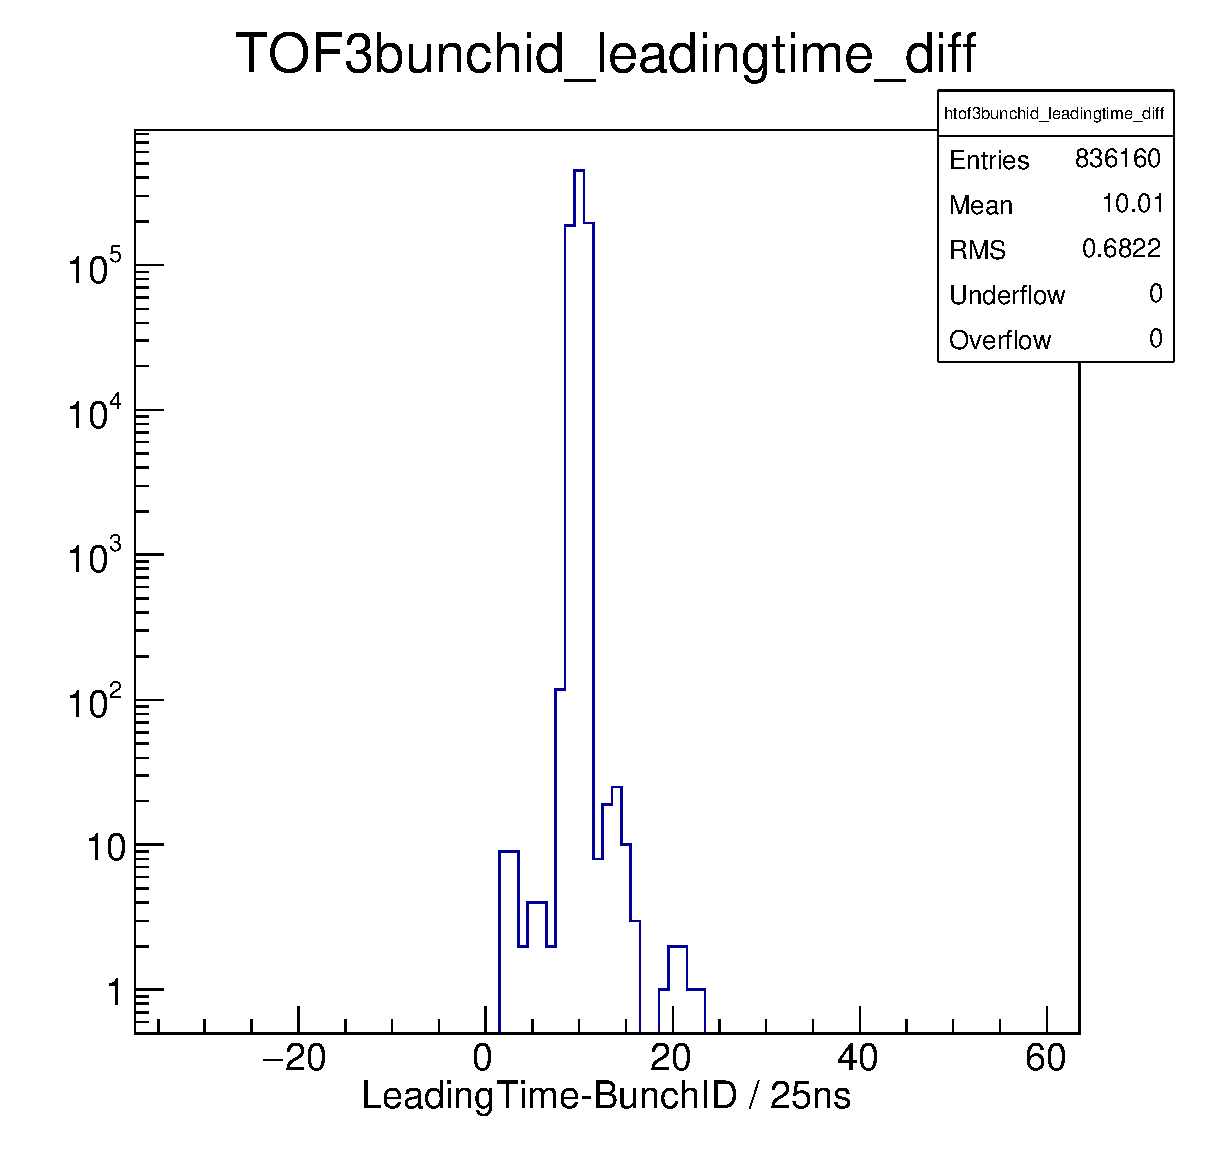
\includegraphics[width=\textwidth]{fig/tof_leadingtime_bunchid_diff.eps}
        \caption{TOF板Leading Time与Bunch ID之差的典型分布}
    \end{subfigure}
    \begin{subfigure}[b]{0.48\textwidth}
        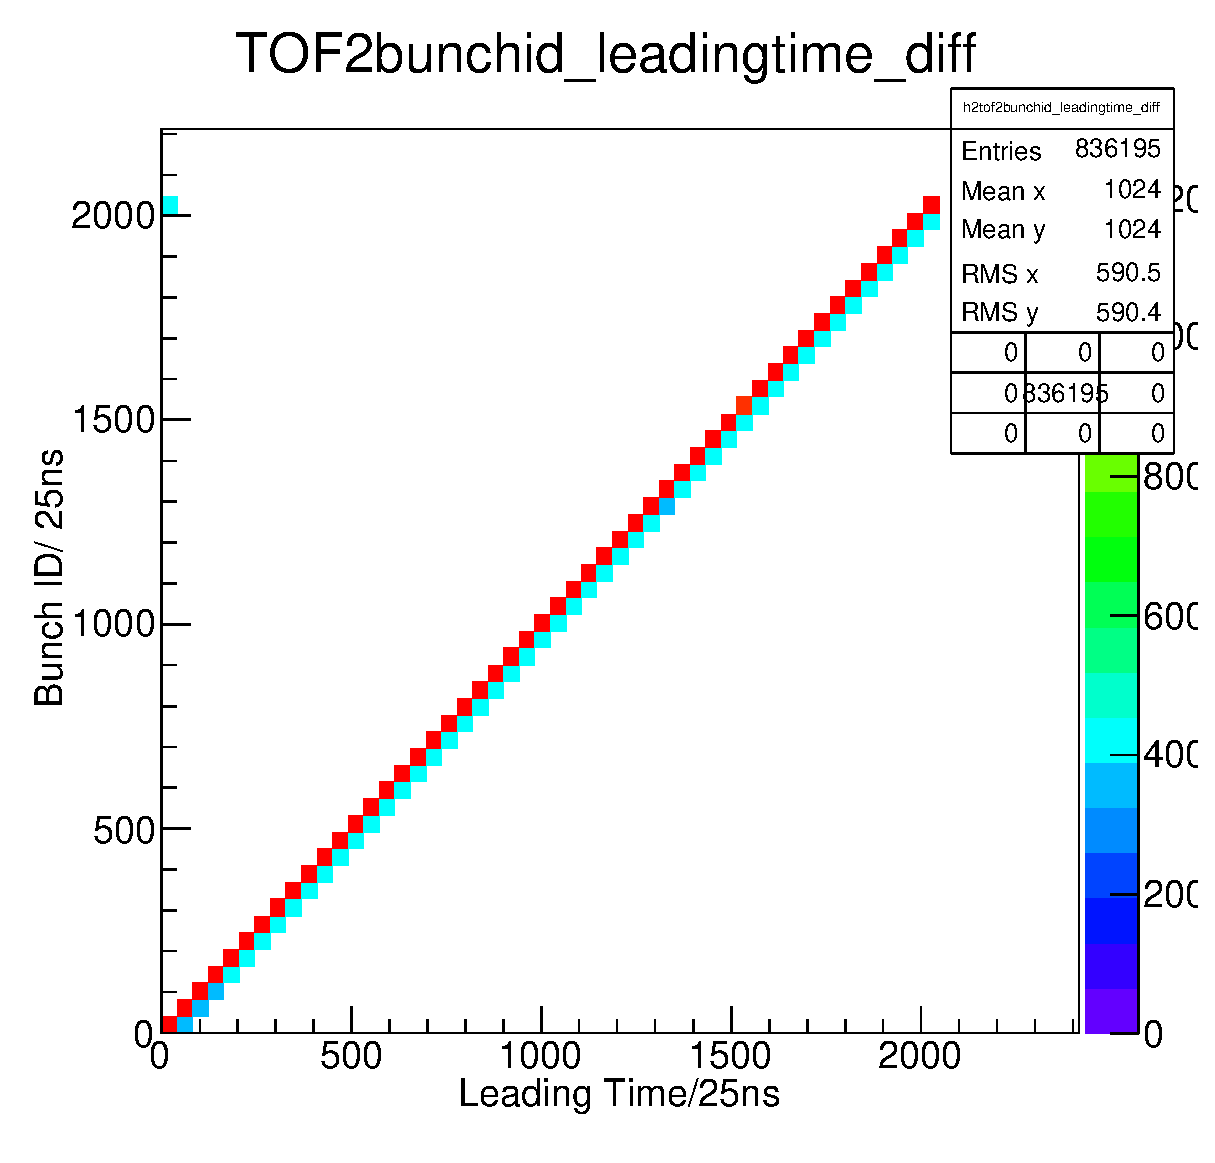
\includegraphics[width=\textwidth]{fig/tof_leadingtime_vs_bunchid.eps}
        \caption{TOF板Leading Time与Bunch ID的关联图}
    \end{subfigure}
	\caption{Leading Time与Bunch ID的关系}
	\label{fig:tof_leadingtime_bunchid}
\end{figure}

\section{获取卡间的时间同步(Time and event synchronization among different DAQ cards)}
\subsection{结果}
\subsubsection*{Event ID}
每块获取卡的Event ID是连续的,没有出现丢事件的情况。
大部分获取卡的起始Event ID为零,但偶尔会出现不为零的情况。此时,获取卡间的事件应该仍然是同步的。

\subsubsection*{Bunch ID}

\section{TOF板的无信号通道数}

\section{单通道的多击中数(Multi-hits in a single channel)}

\section{MWDC单个丝面的击中多重数(Multiplicity in a single MWDC wireplane}

\end{document}